\chapter{FM modulation and demodulation}
\section{Modulation}
For a message signal $m(t)$ and carrier $c(t) = A_c \cos(2\pi f_c t)$ the modulated wave is:
\begin{equation*}
s (t) = A_c \cos\left(2\pi f_c t + 2\pi k_f \int_{0}^{t} m(\tau) d\tau\right)
\end{equation*}
Where $k_f$ is known as \textit{frequency sensitiviy}.
In the case of single tone modulation, where $m(t) = A_m \cos(2\pi f_m t)$ or $m(t) = A_m \sin(2\pi f_m t)$ :

\begin{align*}
	s (t) &= A_c \cos\left(2\pi f_c t + 2\pi k_f \int_{0}^{t} A_m\cos(2\pi f_m \tau) d\tau\right) \\
	&= A_c \cos\left(2\pi f_c t + \frac{2\pi k_f A_m}{2\pi f_m} \sin(2\pi f_m \tau) \right) \\
	s(t) &= A_c \cos\left(2\pi f_c t + \frac{k_f A_m}{f_m} \sin(2\pi f_m \tau) \right)
\end{align*}

Here $k_f A_m = \Delta f$ is called  \textit{frequency deviation} and $\dfrac{k_f A_m}{f_m} = \dfrac{\Delta f}{f_m} = \beta$ is called modulation index.

For a general message signal $m(t)$, modulation index can be defiend as (as far as I looked up in various sources):

$$\beta = \frac{k_f\cdot m_{peak}}{f_{max}}$$

where $f_{max}$ is maximum frequency component present in the message signal. And $m_{peak}$ is peak value of input signal:
$$m_{peak} = \frac{\max\left[m(t) \right] - \min\left[m(t) \right]}{2}$$
You can see that for a simple sine wave with amplitude $A_m$ this just reduces to $m_{peak} = A_m$.

\note{There are some differences in how $\beta$ is defined in various sources.
Here, I've used one of such definitions. (see \textit{page 212, Modern Digital and Analog Communication Systems, B.P. Lathi})}

\section{Demodulation}
Demodulation is done by finding Hilbert transform of FM, extracting instantaneous phase from it and differentiating it (minus phase offset due to carrier):
Hilbert transform: 
$$z = \mathcal{H}(s(t))$$
Instantaneous phase angle (obtained by \mintinline{matlab}|unwrap(angle(z))|)
$$\theta(t) = \measuredangle z(t)$$

Demodulated wave is:
$$m'(t) = \frac{\partial}{\partial t} (\theta(t) - 2 \pi f_c t)$$

\section{Program for narrow and wide band FM modulation and demodulation}
Narrow band FM has $\beta << 1$ and wide band FM has $\beta >> 1$

To modulate at a particular value of $\beta$, $k_f$ has to be found out first
$$k_f =\frac{\beta f_{max}}{m_{peak}}$$

But i don't think, this level of perfection is required in lab exam - they didnt ask for details of how it was implemented.
In the program I've done this anyway. To integrate message signal cumulative summer \mintinline{matlab}|cumsum(m)| is used.

The message signal chosen here is: $m(t) = \sin(2 \pi f_m t) + \sin(4 \pi f_m t)$. Here $f_{max} = 2f_m$.

\importMLCode{code/fm_mod.m}

\begin{figure}[!ht]
	\centering
	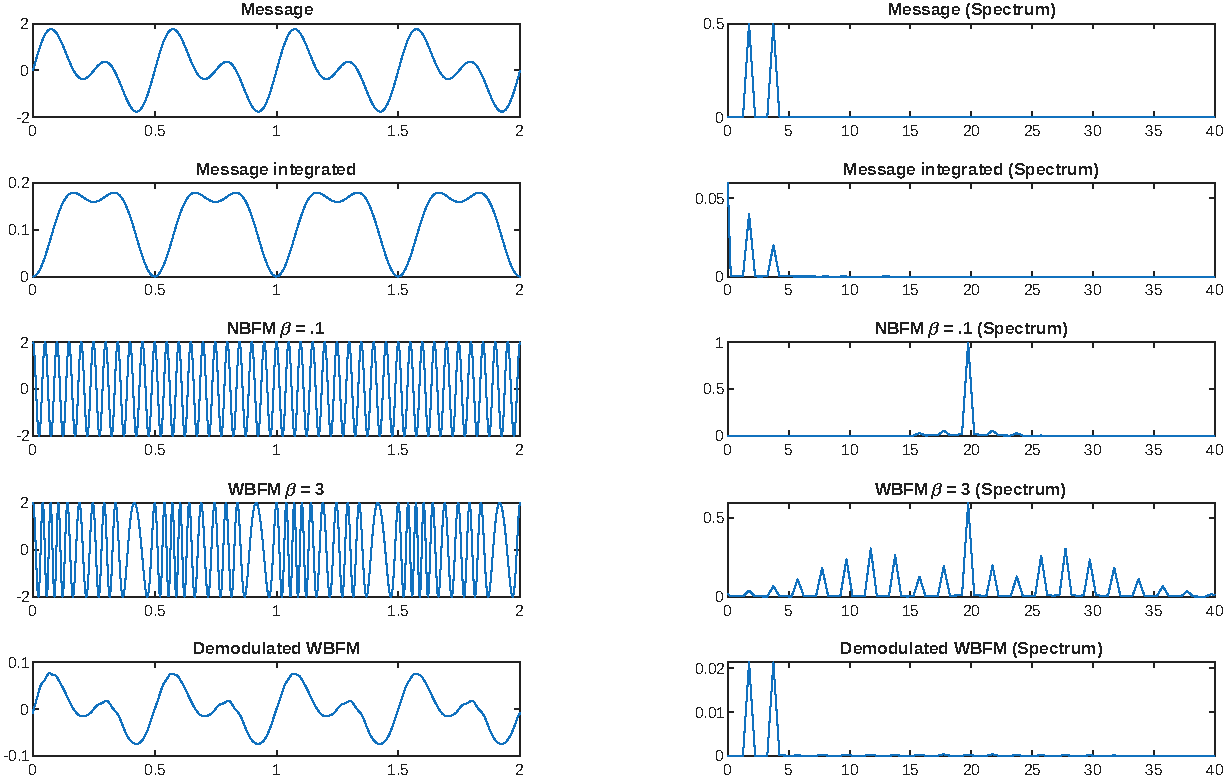
\includegraphics[width=\textwidth]{img/fm.pdf}
\end{figure}

\pagebreak